\documentclass[italian,a4paper]{article}
\usepackage[tight,nice]{units} %unità di misura
\usepackage{babel,amsmath,amssymb,amsthm,graphicx,url,textcomp,gensymb}
\usepackage[text={5.5in,9in},centering]{geometry}
\usepackage[utf8x]{inputenc}
\usepackage[T1]{fontenc}
\usepackage{ae,aecompl}
\usepackage[small,bf]{caption}
\frenchspacing
\pagestyle{plain}
%------------- eliminare prime e ultime linee isolate
\clubpenalty=9999%
\widowpenalty=9999
%--- definizione numerazioni
\renewcommand{\theequation}{\thesection.\arabic{equation}}
\renewcommand{\thefigure}{\arabic{figure}}
\renewcommand{\thetable}{\arabic{table}}
\addto\captionsitalian{\renewcommand{\figurename}{Grafico}}
%------------- ridefinizione simbolo per elenchi puntati: en dash
\renewcommand{\labelenumi}{\textbf{\arabic{enumi}.}}
\renewcommand{\labelitemi}{\textbf{- }}
\setlength{\abovecaptionskip}{\baselineskip}   % 0.5cm as an example
\setlength{\floatsep}{2\baselineskip}
\setlength{\belowcaptionskip}{\baselineskip}   % 0.5cm as an example
%--------- comandi insiemi numeri complessi, naturali, reali e altre abbreviazioni
\renewcommand{\leq}{\leqslant}
%--------- porzione dedicata ai float in una pagina:
\renewcommand{\textfraction}{0.05}
\renewcommand{\topfraction}{0.95}
\renewcommand{\bottomfraction}{0.95}
\renewcommand{\floatpagefraction}{0.35}
\setcounter{totalnumber}{5}
%-------------------------ambiente codice
\usepackage{listings}
\lstset{language=C++,inputencoding=utf8,breaklines=true,extendedchars=true, basicstyle=\small, columns=flexible, linewidth=\textwidth, lineskip=1pt, breakatwhitespace=true, lastline=99999, showstringspaces=false}
\lstloadlanguages{C++}
%-----------------------elenco compatto
\newenvironment{packed_enum}{
\begin{itemize}
  \setlength{\itemsep}{1pt}
  \setlength{\parskip}{0pt}
  \setlength{\parsep}{0pt}
}{\end{itemize}}
%------------shortcuts
\newcommand{\D}{\Delta}
\newcommand{\g}{\gamma}
\newcommand{\w}{\omega}
\newcommand{\f}{\phi}

%---------
%
%---------
\begin{document}
\title{Dinamica molecolare}
\author{\normalsize Ilaria Brivio (582116)\\%
\normalsize \url{brivio.ilaria@tiscali.it}%
\and %
\normalsize Matteo Abis (584206)\\ %
\normalsize \url{webmaster@latinblog.org}}
\date{\today}
\maketitle
%------------------
\section{Introduzione teorica al problema fisico}
Vogliamo studiare il moto di una molecola di HCl, fornendo, in particolare, un'approssimazione della frequenza di \textit{stretching} lungo l'asse molecolare.

Approssimiamo la molecola come due masse puntiformi a distanza $r$ l'una dall'altra, tra le quali agisce il potenziale di Morse
\begin{equation*}
\f(r)= -D e^{-a(r-r_0)} \left(2-e^{-a(r-r_0)}\right)
\end{equation*}
dove $D$, $a$, $r_0$ sono opportune costanti. Nella nostra analisi impiegheremo sempre i seguenti valori:
\begin{equation*}
D=\unit[0.1679]{a.u.} \qquad a=\unit[0.963]{a.u.} \qquad r_0=\unit[2.409]{a.u.}
\end{equation*}

Dallo studio analitico di $\f(r)$ si vede facilmente che:
\begin{packed_enum}
\item quando $r\rightarrow\infty$ $\f$ va a zero asintoticamente a $-2D e^{-a(r-r_0)}$
\item $\f$ presenta un minimo in $r=r_0$, che corrisponde dunque alla distanza interatomica di equilibrio attorno alla quale avvengono le vibrazioni.
\item la forza agente su ogni atomo \`e 
\begin{equation*}
F(r)=-\dfrac{d\f(r)}{r}= 2Da e^{-a(r-r_0)}\left(e^{-a(r-r_0)}-1\right)
\end{equation*}
nulla per $r=r_0$, e di richiamo (ovvero con segno opposto a $r-r_0$) negli altri casi.
\end{packed_enum}

Eseguiremo una simulazione della dinamica della molecola di HCl basata sull'integrazione col metodo di Verlet delle equazioni del moto relativo:
\begin{align*}
\dot{r}&=v\\
\dot{p}&=F(r)=2Da e^{-a(r-r_0)}\left(e^{-a(r-r_0)}-1\right)
\end{align*}

In una prima fase del lavoro confronteremo le approssimazioni ottenute con diversi valori del \textit{time-step} $h$, monitorando l'energia cinetica $K$, l'energia potenziale $V$ e la temperatura istantanea $T=2K \kappa_B$, con $\kappa_B=\unit[3.167 \cdot 10^{-6}]{a.u./K}$.

Fissato poi un $h$ opportuno, realizzeremo un plot di $(r-r_0)(t)$ e uno
dello spettro vibrazionale $|\Psi(\omega)|^2$, ottenuto dal calcolo della
trasformata di Fourier discreta di $(r-r_0)(t)$. Dal grafico dello spettro
sar\`a cos\`i immediata l'individuazione della frequenza di vibrazione
$\omega$.

Confronteremo infine il valore trovato con quello sperimentale $\w_s=\unit[8.5\cdot 10^{13}]{Hz}$ e con quello calcolabile analiticamente come segue:

attorno al minimo del potenziale, $r-r_0\simeq0$ e di conseguenza $e^{-a(r-r_0)}\sim(1+a(r-r_0))$. Cos\`i il potenziale di Morse pu\`o essere approssimato a una parabola, e la forza corrispondente sar\`a di tipo armonico:
\begin{align*}
\f(r)&\sim D \left(a^2(r-r_0)^2-1\right)\\
F(r)&\sim -2 D a^2 (r-r_0)
\end{align*}
Considerando il sistema della molecola come due masse $m_H=\unit[1836]{a.u.}$, $m_{Cl}=\unit[65092]{a.u.}$ collegate da una molla di costante elastica $2Da^2$ si ha
\begin{equation*}
\w_a=\dfrac{1}{2\pi}\sqrt{\dfrac{2Da^2}{\mu}}=\dfrac{1}{2\pi}\sqrt{2Da^2 \dfrac{m_H + m_{Cl}}{m_H m_{Cl}}}\simeq \unit[8.69 \cdot 10^13]{Hz}
\end{equation*}


\section{Algoritmi utilizzati}
\subsection*{Verlet}
Consideriamo un'equazione differenziale della forma $\ddot{x}=F(x_t,t)$. Nel nostro caso, posto $x=r-r_0$, abbiamo:
\begin{equation*}
 \ddot{x}=F(x_t)= 2Da e^{-ax_t}\left(e^{-ax_t}-1\right)
\end{equation*}

Per integrare l'equazione suddividiamo l'intervallo $[0,t]$ in $N$ intervallini di ampiezza arbitraria $h$ e costruiamo un procedimento ricorsivo che dia il valore di $x$ in $t+h$ come funzione di quello in $t$.

La formula ricorsiva di Verlet, che fornisce un'approssimazione a meno di termini del quarto ordine in $h$ per $x$ e del secondo ordine per $v$ si scrive:
\begin{align*}
x(t+h)&= 2 x(t) -x(t-h) + h^2 F(x(t)) +\mathcal{O}(h^4)\\
v(t)&=\dfrac{x(t+h)-x(t-h)}{2h} +\mathcal{O}(h^2)
\end{align*}

In questo modo per calcolare $x(T)$, \`e sufficiente iterare l'algoritmo $N=T/h$ volte dall'istante iniziale. L'approssimazione sar\`a naturalmente tanto pi\`u vicina alla soluzione analitica quanto pi\`u grande \`e $N$, e quindi pi\`u piccolo \`e $h$.

% L'algoritmo di Verlet \`e stato incluso nel file \texttt{verlet.cpp}:\\
\subsection*{Trasformata di Fourier discreta (DFT)}
Consideriamo una funzione $y$ periodica di periodo $T$. Suddividiamo tale intervallo temporale in $N+1$ intervallini di ampiezza $h$, cos\`i che $T=Nh$ e $y_k=kh$. 
Supponiamo di conoscere il valore della funzione solo nei punti discreti $y_k=y(t_k)$ e vogliamo calcolare lo sviluppo in serie di Fourier di $y(t)$ nelle frequenze discrete $\w_n=n 2\pi/T=n 2Pi/Nh$. 

Utilizzando la regola di integrazione trapezoidale, possiamo approssimare la trasformata $Y(\w)$ con una serie di $N$ termini:
\begin{equation*}
Y(t)=\dfrac{1}{\sqrt{2\pi}}\int_{-\infty^\infty}{e^{i\w t}y(t)dt} \simeq \dfrac{h}{\sqrt{2\pi}}\sum_{n=1}^{N}{y_k e^{2\pi i\w_n}}=h\sum_{n=1}^N{Y(\w_n)}
\end{equation*}
In questo modo, riscrivendo gli esponenziali in termini di seni e coseni si ottengono le espressioni seguenti:
\begin{align*}
y_k&=\dfrac{\sqrt{2\pi}}{N}\sum_{n=1}^N{\left[\cos(nk\theta)\Re Y_n+\sin(nk\theta)\Im Y_n + i\left(\cos(nk\theta)\Im Y_n - \sin(nk\theta)\Re Y_n\right)\right]}\\
Y_n&=\dfrac{1}{\sqrt{2\pi}}\sum_{k=1}^N{\left[\cos(nk\theta)y_k+i\sin(nk\theta)y_k\right]}
\end{align*}
dove si \`e posto $\theta=2\pi/N$. Si osservi che l'algoritmo ottenuto d\`a una buona approssimazione della trasformata di Fourier solo pre frequenze inferiori a $\w_{\max}=\w_N=2\pi/h$; si considera sempre implicitamente $n=1,\dots, N$.

In particolare l'andamento di $Y_n$ fornir\`a la composizione dello spettro di $y$ in termini delle frequenze $\w_n$.

\section{Risultati ottenuti}

Abbiamo eseguito la simulazione con l'algoritmo di Verlet per un tempo $T =
10000$ con passi di $h = 0.01$, che sono molto più piccoli del periodo, come
si vede dai grafici. L'evoluzione della posizione nel tempo risulta:
 \begin{figure}[h!]
 \begin{center}
 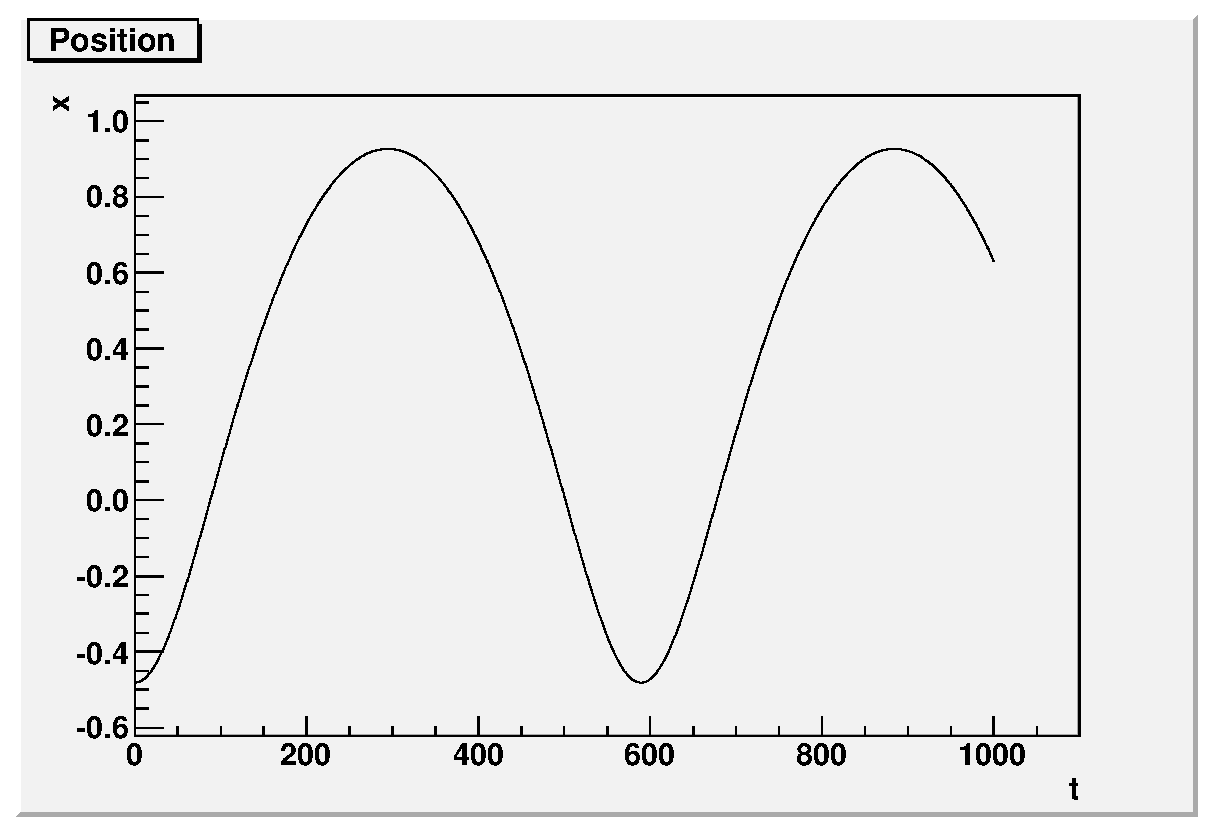
\includegraphics[width=0.77\textwidth]{position_graph.eps}
 \caption{
 }
 \label{}
 \end{center}
 \end{figure}

 Si nota che l'algoritmo è stabile, infatti l'energia oscilla poco intorno
 al valore iniziale:
 \begin{figure}[h!]
 \begin{center}
 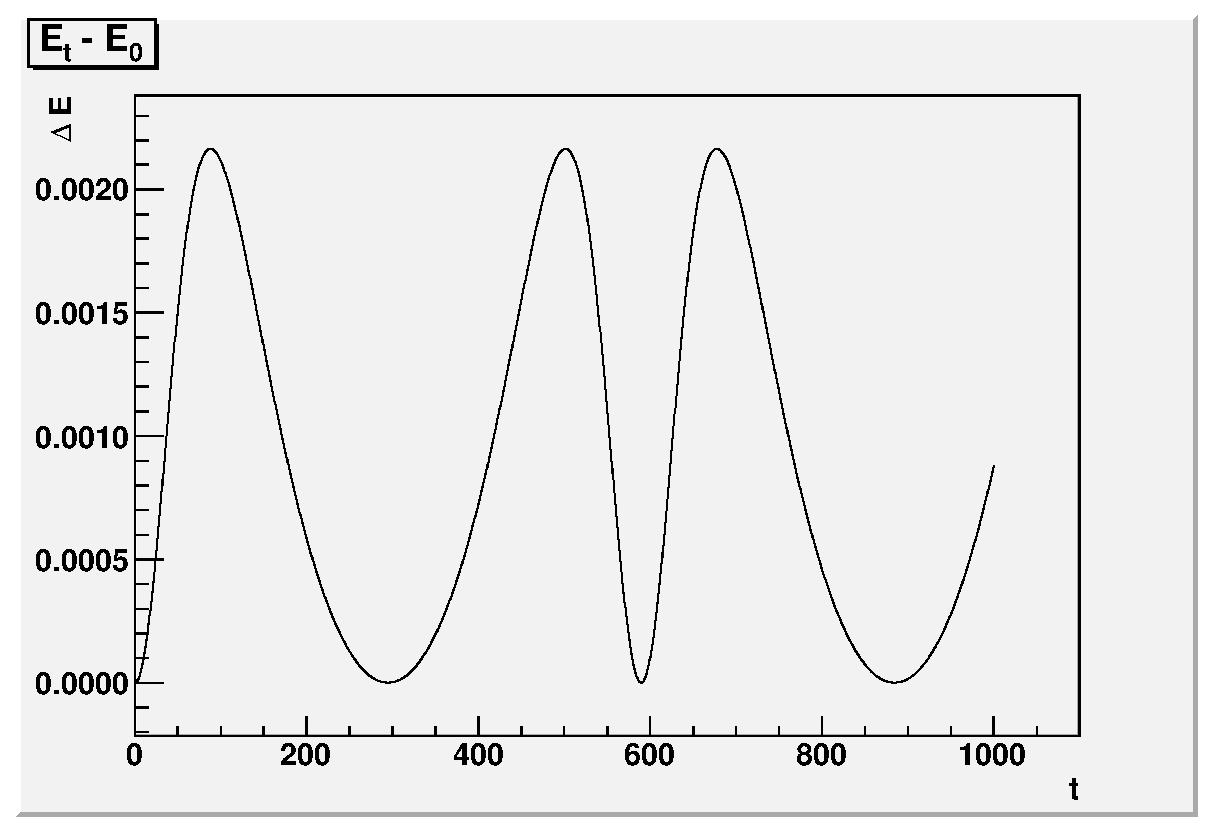
\includegraphics[width=0.77\textwidth]{delta_energy_graph.eps}
 \caption{
 }
 \label{}
 \end{center}
 \end{figure}

\clearpage
\section{Programmi utilizzati}

% \lstinputlisting{}
% \newpage


\end{document}
